\documentclass[sigconf,authorversion,nonacm]{acmart}

\usepackage{minted}
\usemintedstyle{borland}
\setminted{linenos=true,fontsize=\normalsize}

\usepackage{fontspec}
\setmonofont{Fira Code Retina}[Scale=MatchLowercase]

\captionsetup{justification=centering, margin=1cm}

\AtBeginDocument{%
  \providecommand\BibTeX{{%
    \normalfont B\kern-0.5em{\scshape i\kern-0.25em b}\kern-0.8em\TeX}}}

\begin{document}

\title{Tarea 2 \\ Recocido simulado con el problema de $k$ vendendores viajeros}

\author{Mario Emilio Jiménez Vizcaíno}
\email{A01173359@itesm.mx}

\maketitle

\section{Introducción}
El problema del vendedor viajero (o mejor conocido como TSP) es un problema famoso por ser muy fácil de describir y difícil de resolver. \cite{hoffman2013traveling} El problema puede plantearse de forma sencilla: si un vendedor ambulante desea visitar exactamente una vez cada una de una lista de ciudades y luego regresar a la ciudad inicial, ¿cuál es la ruta más corta que el vendedor puede tomar?

En esta tarea se aborda una variante de este problema, conocida como "el problema de múltiples vendedores viajeros", o por sus siglas en inglés, mTSP. Esta variate es una generalización del problema, en el que se permite utilizar más de un vendedor en la solución. Por sus características, este problema usualmente es más apropiado a aplicaciones en la vida real.\cite{bektas2006multiple}

\section{Metodología}
Para esta tarea implementé una solución del problema usando el algoritmo de recocido simulado, en el que utilizando parámetros controlados como la temperatura y la longitud de cadena, se corren cadenas de Markov para generar soluciones mejores, o posiblemente no tan mejores, dependiendo de la temperatura del algoritmo.

Algunas de las decisiones que tomé para realizar esta implementación se describen a continuación.

\subsection{Representación de los individuos}
Para representar las $n$ ciudades opté por generar una lista de $0$ a $n-1$, en la que cada número indica el índice de la ciudad a la que el viajero se moverá a continuación. Para asegurarme que las listas fueran soluciones válidas al problema consideré dos restricciones principales:
\begin{itemize}
  \item Que la función de mutación sólo intercambie números de lugar en vez de generar nuevos.
  \item Que el número de ciclos que formaban los caminos fuera igual al número de vendedores viajeros. Esta validación se lleva a cabo dentro de la función \texttt{is\_solution\_valid}, que llama a la función \texttt{calculate\_cycle\_number\_map} para generar una lista de la misma longitud que la solución, pero con el índice del ciclo al que pertenece la ciudad, y después obtener el índice máximo y compararlo con el número de vendedores viajeros.
\end{itemize}

Un ejemplo de esta representación para un problema de 10 ciudades y 3 vendedores es \texttt{[1 9 5 2 7 4 3 6 8 0]}, y el resultado de \texttt{calculate\_cycle\_number\_map} con esa solución como argumento es \texttt{[0 0 1 1 1 1 1 1 2 0]}, lo que significa que la primera, la segunda y la última ciudad son visitadas por el primer vendedor, el segundo vendedor visita de la ciudad 3 a la 8 y el tercer vendedor visita la novena.

\subsection{Función de evaluación}
La función de evaluación es muy simple: recibe a una solución válida y regresa la distancia necesaria para cubrir los caminos que esta solución representa.

Esta función está compuesta por sólo dos líneas:
\begin{enumerate}
  \item \texttt{rows = np.arange(solution.shape[0])}\\
    Esta línea genera una lista de números del $0$ a $n-1$, siendo $n$ la longitud de la solución
  \item \texttt{return np.sum(self.distances[rows, solution])}\\
    Esta línea aprovecha las propiedades de indexación que \textit{numpy} nos provee, ya que la matriz \texttt{self.distances}, que contiene las distancias entre dos ciudades, es indexada en el eje $x$ por esa lista de números del $0$ a $n-1$, y además indexada en el eje $y$ por la solución, que igualmente es una lista de valores entre $0$ y $n$. Finalmente, esta lista de distancias es sumada usando la función \texttt{np.sum}, y regresada de la función.
\end{enumerate}

\subsection{Función de mutación}
Mi implementación de la función de mutación, \texttt{mutate\_solution}, recibe como parámetro opcional una solución $s1$ y regresa otra solución $s2$.
En caso de que el parámetro de solución $s1$ no sea enviado, se genera una solución "tonta" creando una secuencia de números entre $0$ y $n-1$ (índices de ciudades), en donde $n$ es el número de ciudades y se desordena aleatoriamente.

La función de mutación sólo realiza operaciones de intercambios de números, eligiendo dos índices aleatorios con la función \texttt{generate\_random\_swap} y checando si la solución mutada es válida con la función \texttt{is\_solution\_valid} y que checando que la solución mutada no sea la misma que la solución original (si fue pasada como parámetro).


\section{Resultados}
Para probar la implementación utilicé los siguientes parámetros:
\begin{itemize}
  \item $n\_cities = 30$, generar las coordenadas de 30 ciudades en un mapa de 0 a 1
  \item $n\_salesmen = 6$, el número de vendedores viajeros (o ciclos en mi representación)
  \item $\alpha = 0.8$, el factor por el que se multiplicará la temperatura después de cada cadena de Markov
  \item $\beta = 1.5$, tiene el mismo propósito que $\alpha$, pero es usada durante el ajuste de la temperatura inicial
  \item $n\_batches = 200$, el número máximo de cadenas de Markov a ejecutar
  \item $n\_iterations = 500$, representa el número de iteraciones o soluciones a probar por cada cadena de Markov
  \item $min\_accepted = 0.8$, la fracción de soluciones aceptadas necesaria para que el proceso de ajuste de la temperatura inicial termine
  \item $max\_batches\_with\_same\_solution = 20$, el número de cadenas de Markov que regresen la misma solución necesario para detener el algoritmo ya que no se detecta un avance
\end{itemize}

El tiempo total de ejecución fue de 26.06 segundos, ejecutando 96 cadenas de Markov (las últimas 20 con la misma solución, evaluada en 3.53), cada cadena de 500 posibles soluciones.

La solución final fue graficada en el siguiente mapa:

\begin{figure}[H]
  \centering
  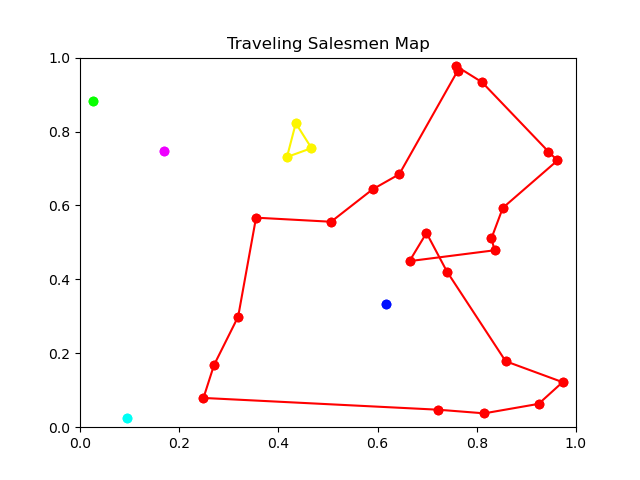
\includegraphics[width=\linewidth]{map.png}
  \caption{Mapa de los vendedores viajeros, en donde cada color representa un viajero diferente}
\end{figure}

\subsection{Curva de mejor encontrado}
La evolución de la evaluación de la mejor solución forma una curva graficada a continuación:

\begin{figure}[H]
  \centering
  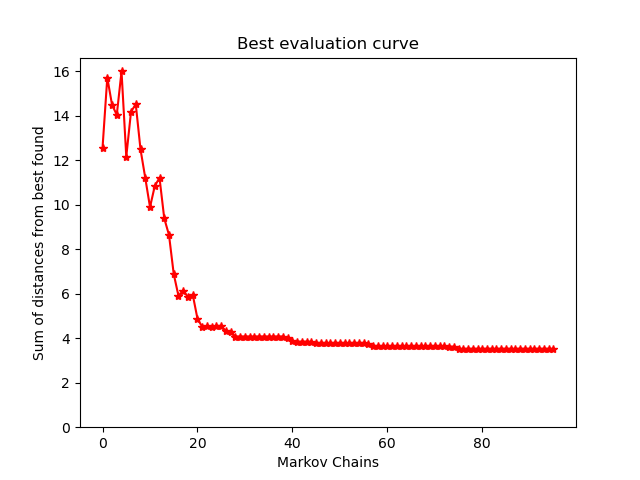
\includegraphics[width=\linewidth]{curve.png}
  \caption{Curva de mejor encontrado para el mapa anterior}
\end{figure}

En el inicio se puede observar que en ocasiones la cadena de Markov acepta soluciones peores (visualizadas como saltos hacia arriba, ya que se elige una solución con una evaluación más alta que la anterior) como consecuencia de que la temperatura es inicializada con el valor de 2.56, pero conforme el algoritmo avanza y la temperatura disminuye se eliminan los saltos hacia arriba.

\section{Conclusión y retos encontrados}
Considero que la implementación del problema de múltiples vendedores viajeros utilizando el algoritmo de recocido simulado tuvo resultados decentes, a pesar de que se pueden observar algunos cambios "obvios" a simple vista. Definitivamente fue un ejercicio enriquecedor para entender experimentalmente cómo funciona este algoritmo, además de poder mejorar mis habilidades en Python.

Entre los retos que enfrenté, los que considero más interesantes fueron:
\begin{itemize}
  \item Aprendí sobre el perfilado de programas en Python, lo que fue útil para mejorar la función \texttt{calculate\_cycle\_number\_map}, que originalmente estaba implementada con el algoritmo DFS (lineal sobre el tamaño de la solución), y que después descubrí era muy tardada ya que era ejecutada directamente por el intérprete de Python, por lo que la cambié por una implementación que usa \texttt{np.min} y que de hecho tiene una complejidad de tiempo cuadrática, pero como está mucho mejor optimizada y a parte la entrada es pequeña, por lo que tiene un desempeño mejor.
  \item Mejoré mi entendimiento de la librería \textit{matplotlib}, que ya había utilizado para crear gráficas anteriormente, pero esta tarea me permitió experimentar con los mapas de colores, las gráficas múltiples usando la misma figura y el manejo de los datos que esperan las funciones como \texttt{plt.plot} y \texttt{plt.scatter}.
\end{itemize}


\bibliographystyle{ACM-Reference-Format}
\bibliography{references}

\clearpage

\appendix

\begin{figure*}
  \section{Implementación del problema de Múltiples Vendedores Viajeros en Python}
  \inputminted[lastline=50]{python}{/home/mario/git/MarioJim/ITC-Tec/Sem7/InteligenciaComp/RecocidoSimulado/A01173359_T2.py}
\end{figure*}

\begin{figure*}
  \inputminted[firstline=52,lastline=105]{python}{/home/mario/git/MarioJim/ITC-Tec/Sem7/InteligenciaComp/RecocidoSimulado/A01173359_T2.py}
\end{figure*}

\begin{figure*}
  \inputminted[firstline=107,lastline=159]{python}{/home/mario/git/MarioJim/ITC-Tec/Sem7/InteligenciaComp/RecocidoSimulado/A01173359_T2.py}
\end{figure*}

\begin{figure*}
  \inputminted[firstline=162]{python}{/home/mario/git/MarioJim/ITC-Tec/Sem7/InteligenciaComp/RecocidoSimulado/A01173359_T2.py}
\end{figure*}

\end{document}
\endinput